\documentclass{article}
\usepackage{graphicx}

\newcommand{\Csharp}{%
  {\settoheight{\dimen0}{C}C\kern-.05em \resizebox{!}{\dimen0}{\raisebox{\depth}{\#}}}}

\begin{document}
\title{COMP6205 Web Development\\}
\author{Group 8\\Shantnu Singh - ss18g15\\Doug Morgan - dm3g14}
\date{\today}
\maketitle

\section{Overview}
    \par
        The assignment involved creating a prototype for a real-estate website aimed at university students.
        The website needs to allow: landlords to list properties, administrators to approve properties, landlords to be able to track the status of their property, and students to view approved properties.
        We have achieved all of these requirements and have added a number of other useful features, including but not limited to landlords having the ability to edit any details of a property, requiring re-approval by the University officer.

    \par
        Since the project required efficient use of ASP.NET Razor pages, a technology neither of us had used previously used, we decided to begin the project by pair programming, which allowed us to gain an understanding of how the logic of the application would work, and then develop individually later on, each of us working on a set of features.
        This meant that tasks could easily be split between us.

    \par
        To make programming separately easier, we used Git for version control.
        Visual Studio 2017 was the ideal IDE as it had in-build Razor development support, such as; IntelliSense, for code completion; package management, through NuGet and deployment to Azure.
        An SQL Express database was used and initialised through migrations created using the IDE.

\section{Design}
    \par
        Before we could start programming, some thought had to be given to the design of the user interface and database.
        We did this on pen and paper and using tools such as LucidChart.
        The logo for the website was also created at this time and other images we used were sourced from the copyright-free section of Google Images.
        The initial design of the website and the final database design is shown in Figures \ref{fig:early_sketches} and \ref{fig:sql_tables}.

        \begin{figure}[ht]
            \centering
            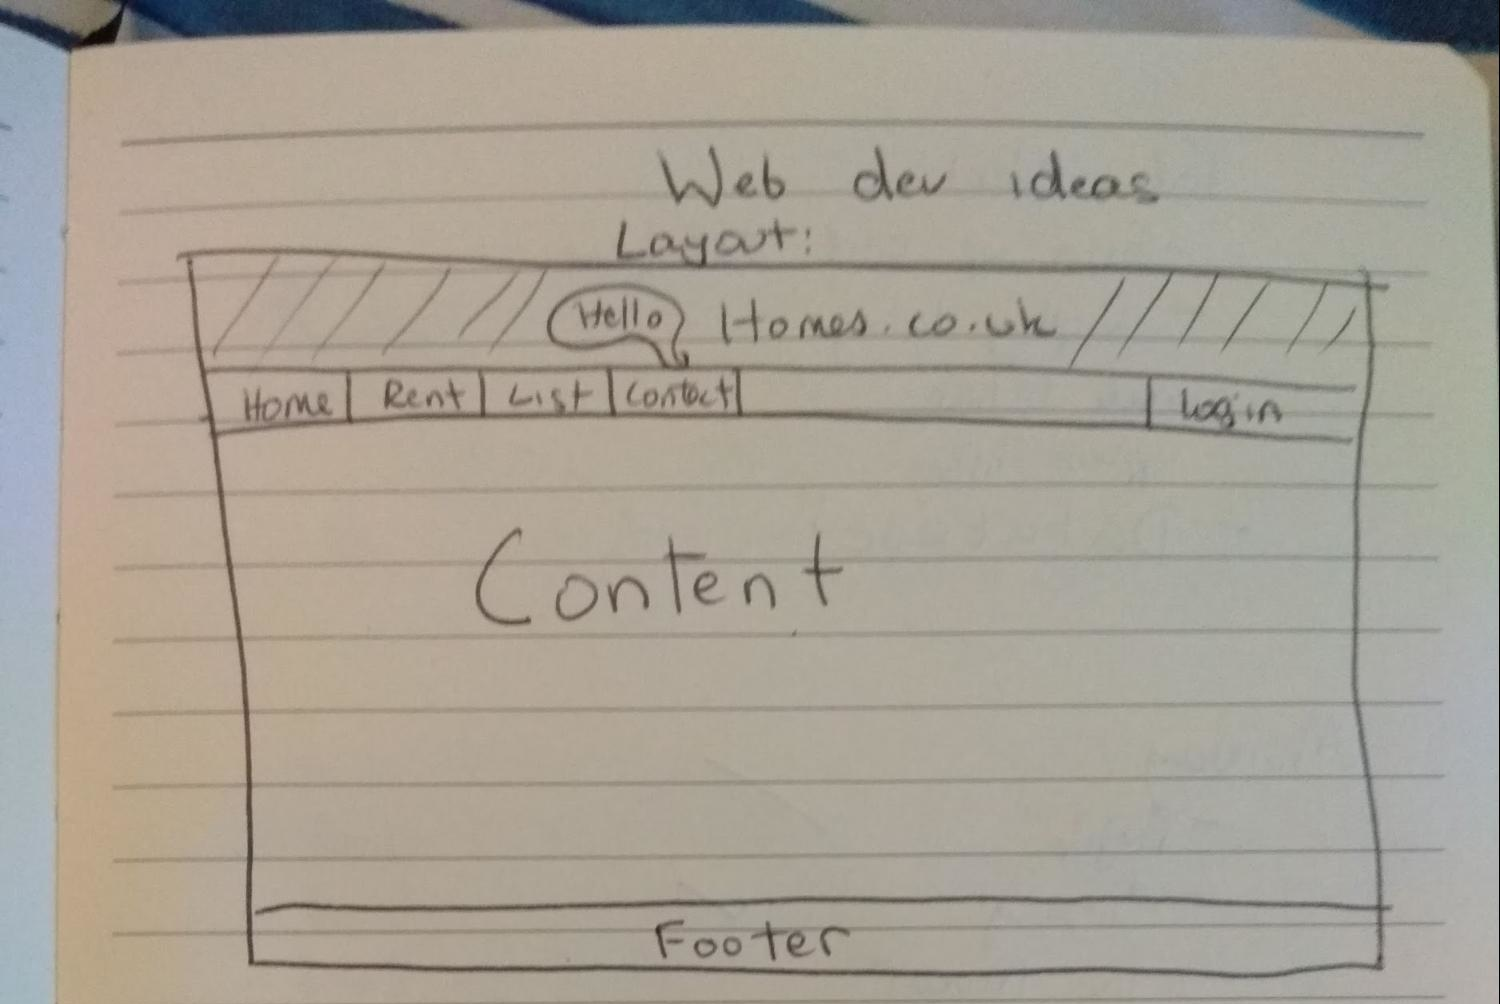
\includegraphics[width=0.48\textwidth]{figures/layout_sketch1.png}
            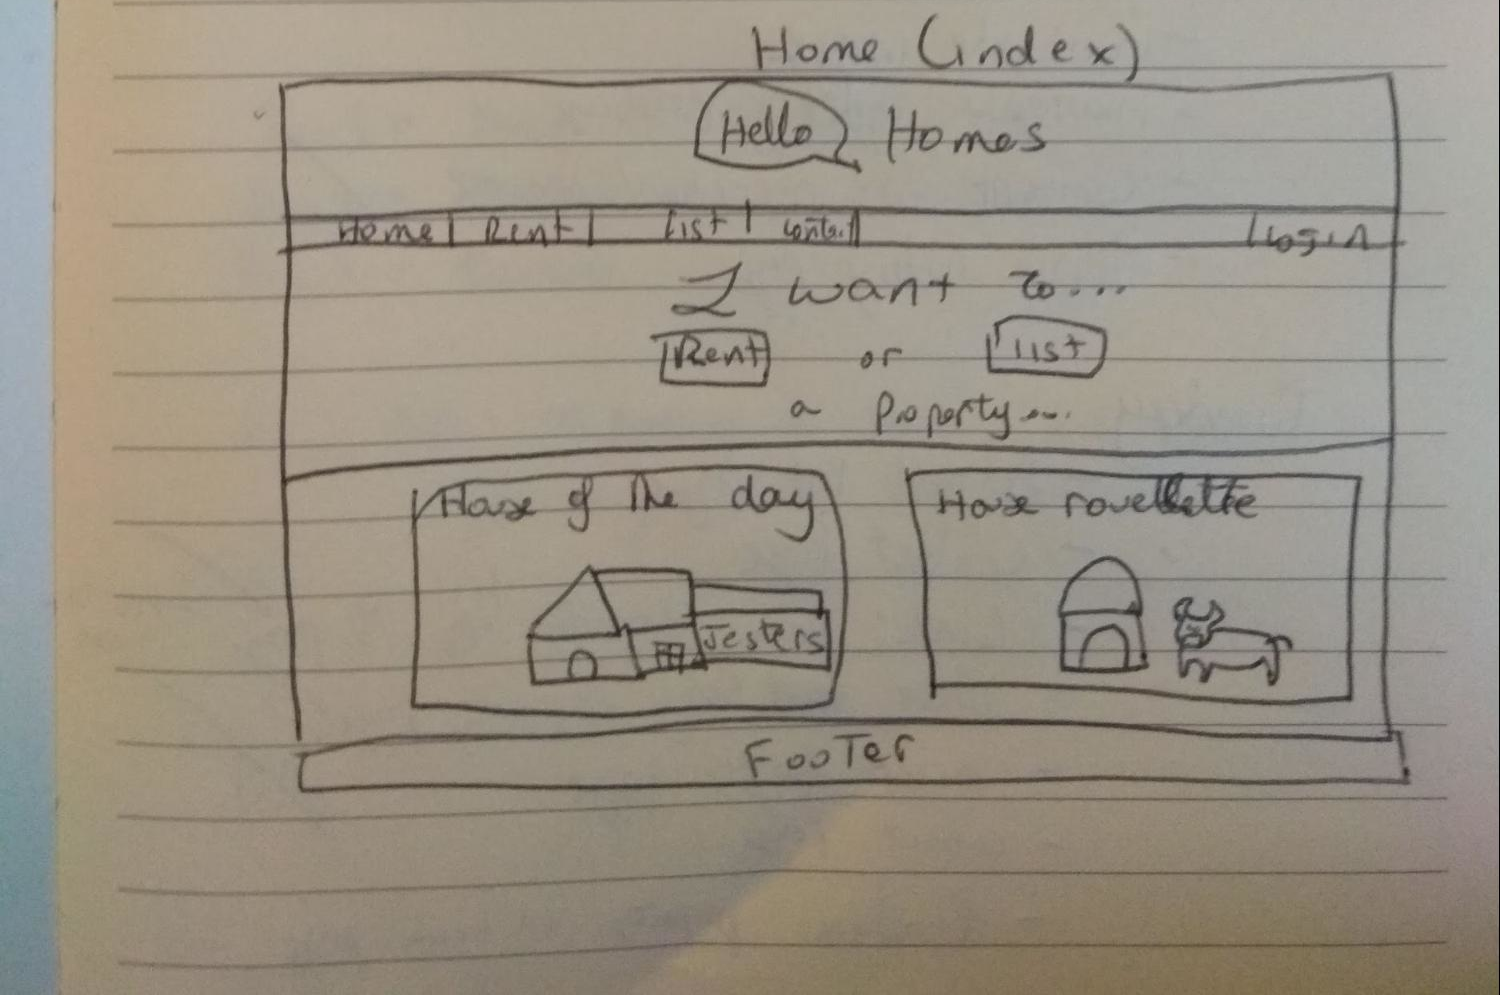
\includegraphics[width=0.48\textwidth]{figures/layout_sketch2.png}
            \caption[Early Sketches]{Early sketches of the web interface}
            \label{fig:early_sketches}
        \end{figure}

        \begin{figure}[ht]
            \centering
            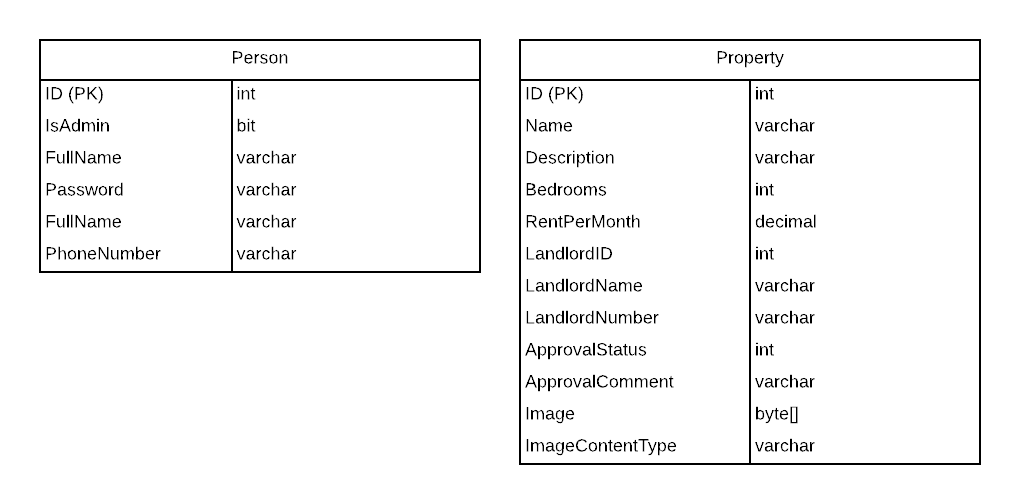
\includegraphics[width=\textwidth]{figures/sql_tables.png}
            \caption[SQL Tables]{Tables used in the final SQL database}
            \label{fig:sql_tables}
        \end{figure}

    \par
        When designing user accounts, consideration was given to all site users having an account, with different authorisation levels representing student, landlord and administrator.
        However, the student never needs to interact with the site in a way that would benefit from being logged into it, so it seemed more sensible to limit to only two kinds of user account: user and admin.
        A signed in user is able to post and edit property listings, and to see the approval status of their listings.
        An admin is able to approve or reject listings, and are required to give a brief comment in either case.
        Users who are not signed in have no capability to list properties or to view properties that have not been approved.

    \par
        The visual design has been achieved using Bootstrap, an HTML and CSS library which provides dynamically resizable elements.
        We chose this tool for greater visual consistency over manually defined parameters, as it allows portable layouts to be defined easily, so that the site can be effectively viewed on all devices.

        \begin{figure}[ht]
            \centering
            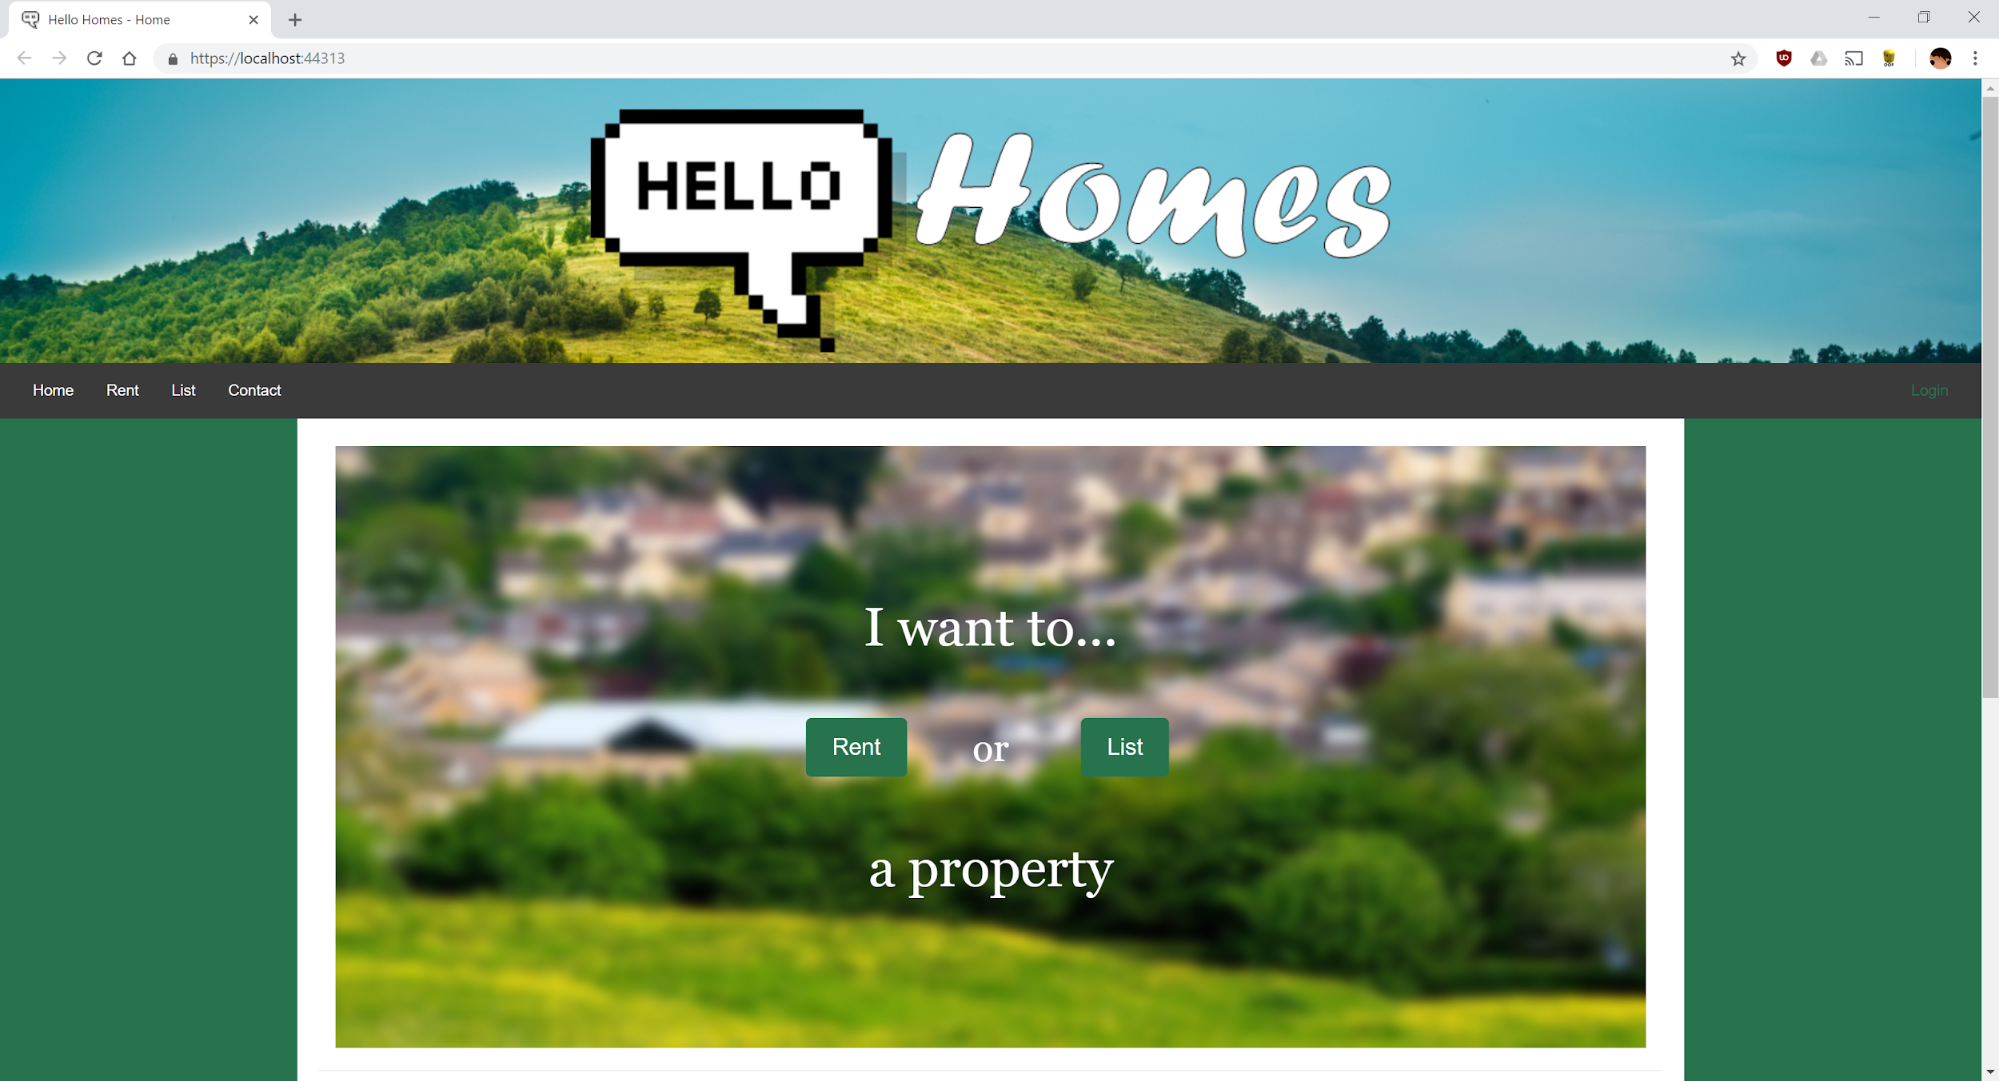
\includegraphics[width=\textwidth]{figures/index_page.png}
            \caption[Home page layout]{Layout of the home page, designed using Bootstrap}
            \label{fig:index_page}
        \end{figure}

\section{Features}
    \subsection{Main Features}
        \par
            The main features of the website consisted of:
            \begin{itemize}
                \item Ability for all users to view approved properties
                \item Ability for landlords to add new properties
                \item Ability for admins to approve and reject properties
            \end{itemize}

        \par
            In addition to this, there had to be some form of authentication and a separate section for the admin user.

        \par
            Figure \ref{fig:rent_page} shows the page where approved properties are listed.
            Here only the title, image, description and cost of the property is shown, but upon clicking the title of the property, the user is taken to a page where full details, including contact details are shown.

            \begin{figure}[ht]
                \centering
                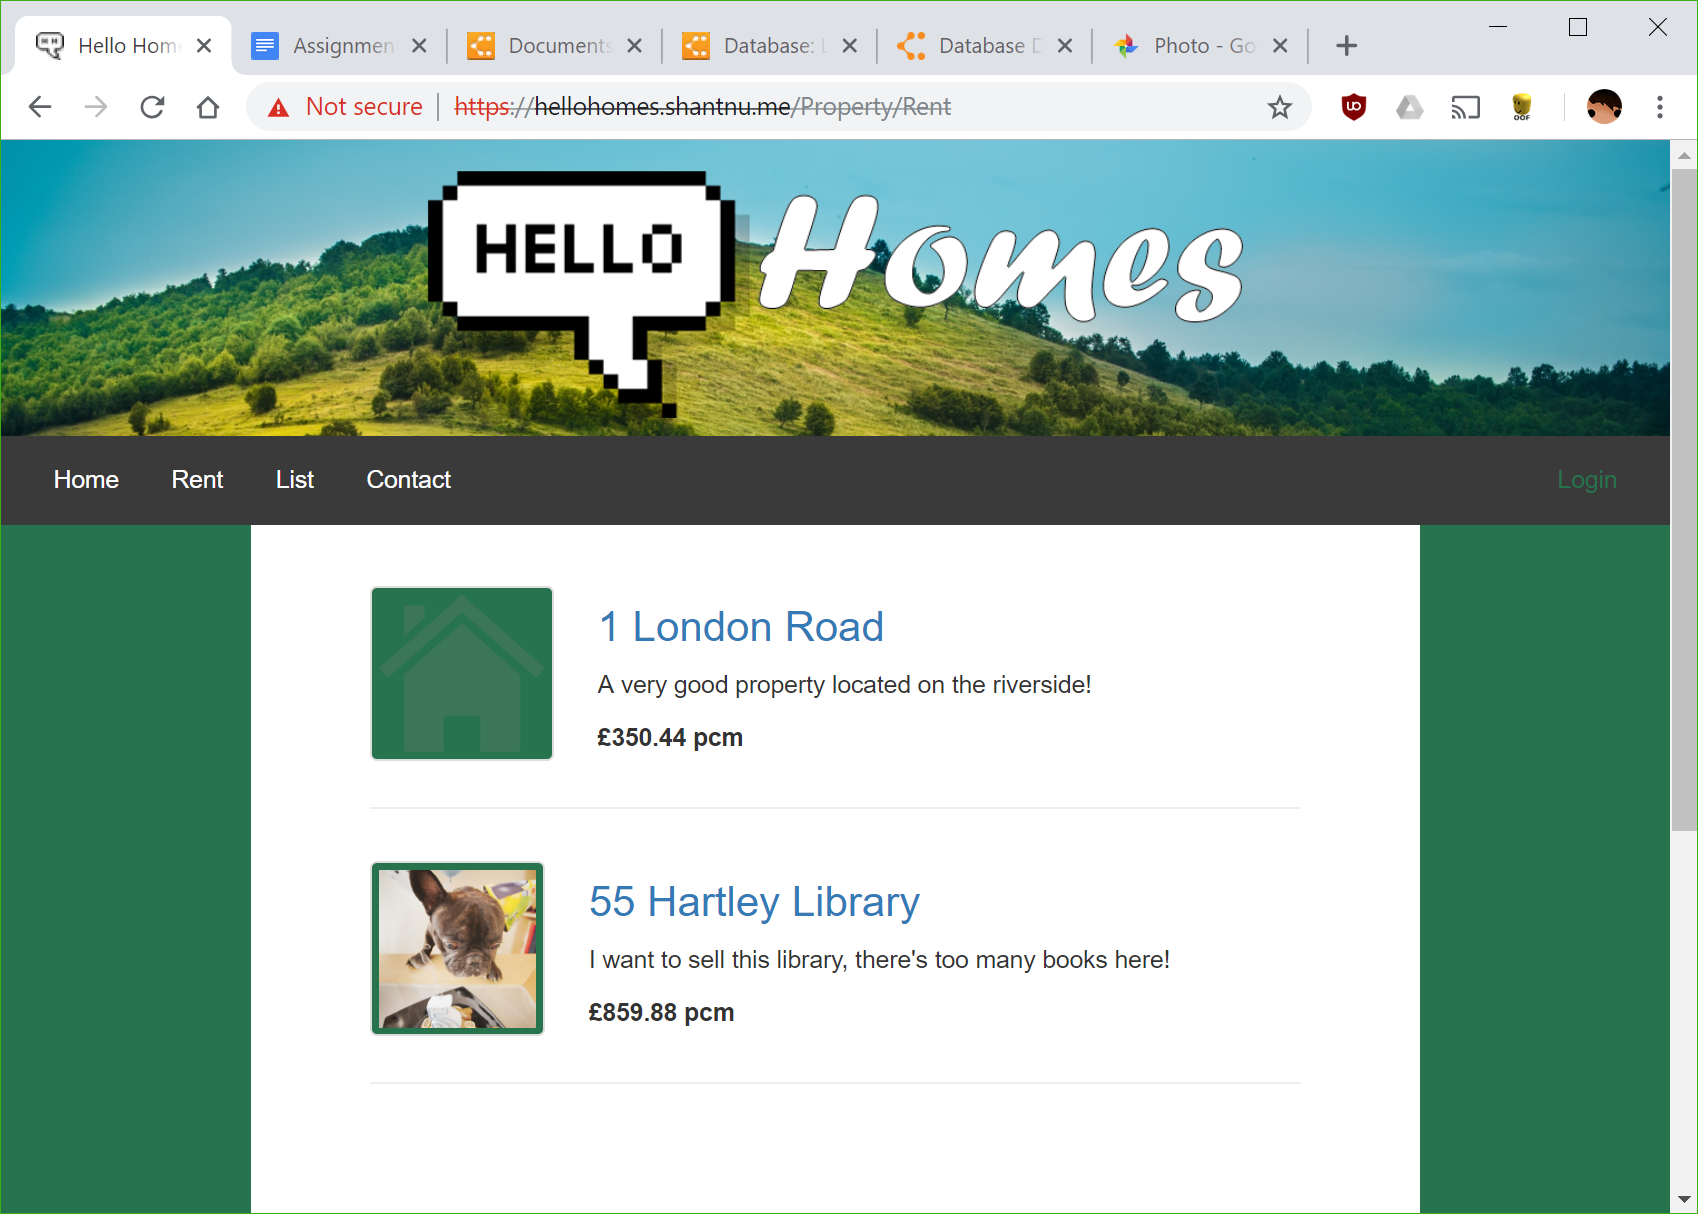
\includegraphics[width=0.7\textwidth]{figures/rent.png}
                \caption[Rent Page]{The rent page, where approved properties appear}
                \label{fig:rent_page}
            \end{figure}

        \par
            The user, after authenticating, can access a page where they can see the properties they have listed and their current approval status.
            They are also shown a comment if the property was approved or rejected.
            On top of this page, there is a button to add a new property.
            Figure \ref{fig:add_property} shows the add property page.

            \begin{figure}[ht]
                \centering
                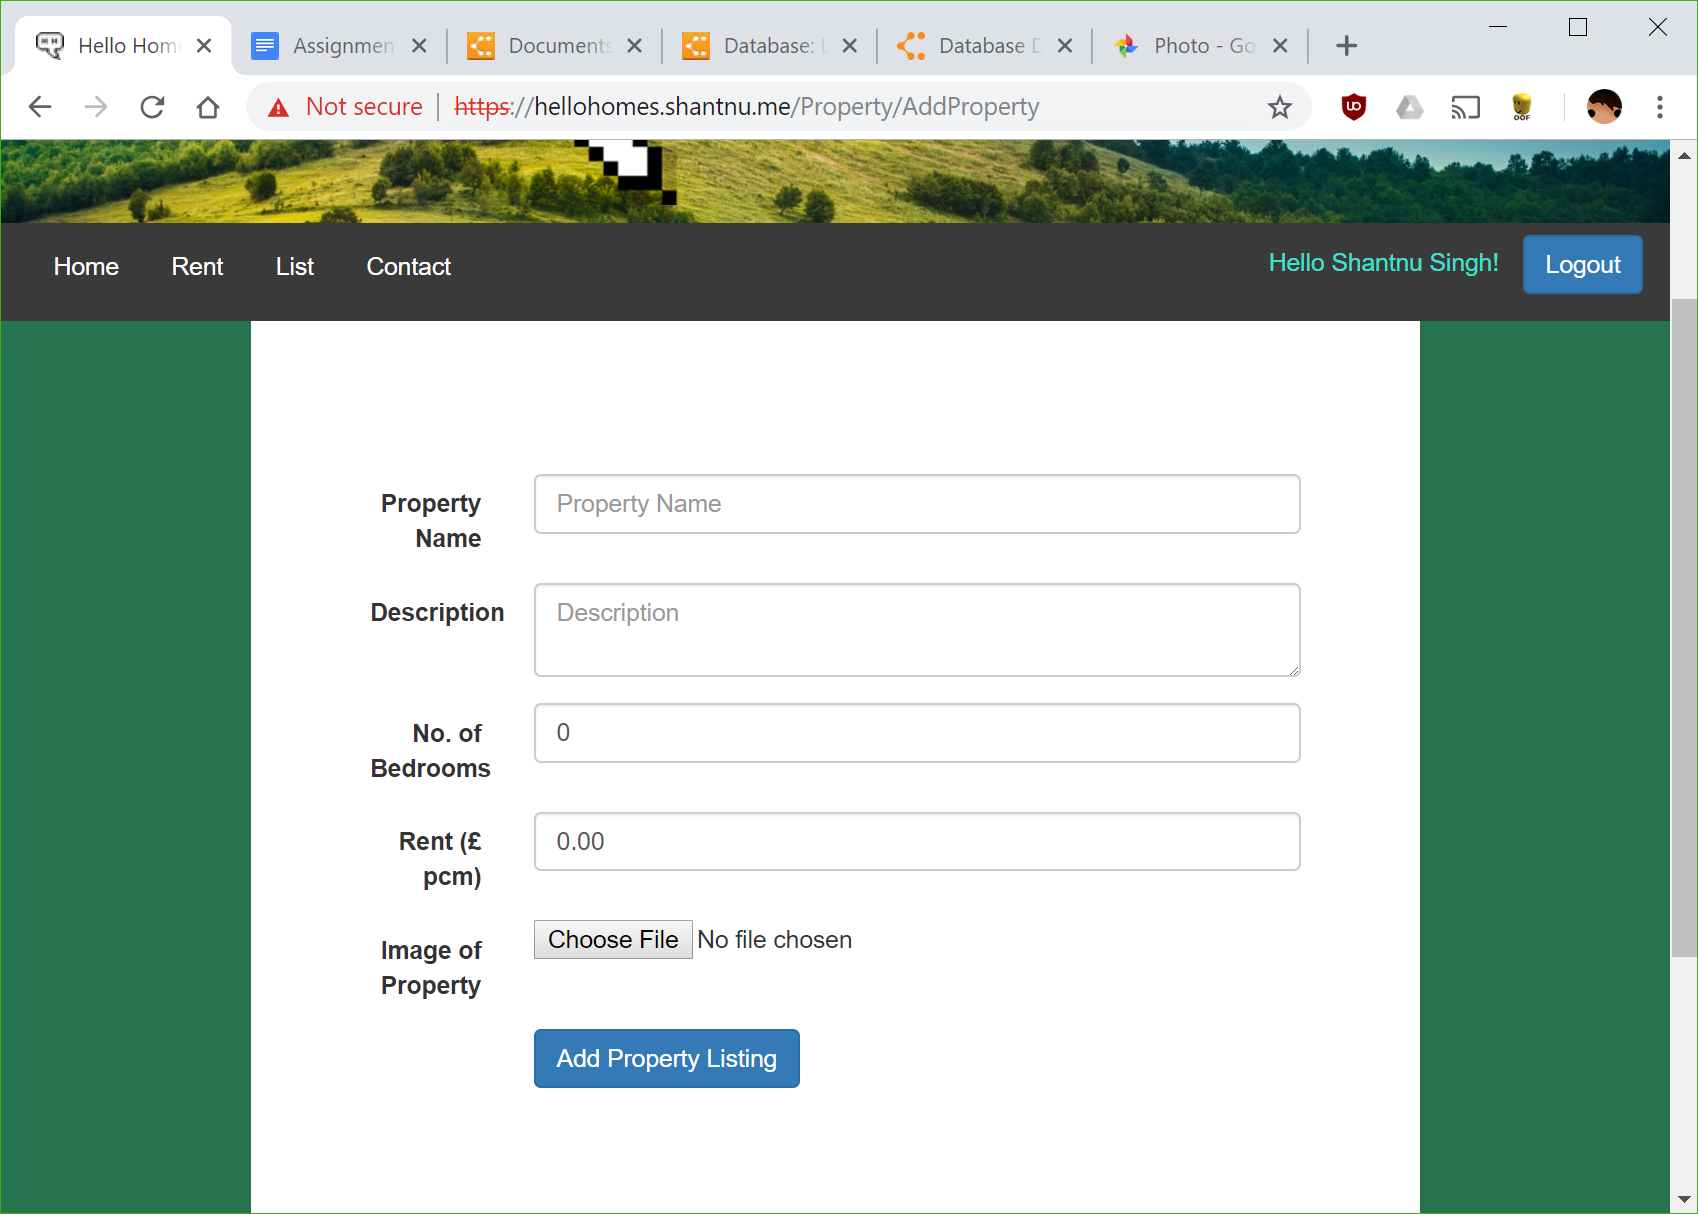
\includegraphics[width=0.7\textwidth]{figures/add_property.png}
                \caption[Add Property]{Adding a property to the listings}
                \label{fig:add_property}
            \end{figure}

        \par
            When a new property is listed (or a current property edited), it must be approved before it is displayed; this can be done in the admin section of the site.
            Each pending property is listed here, along with a button to approve or reject them, as shown in Figure \ref{fig:admin_page}.
            Clicking on either of these options shows the admin details about the property, along with a text box to leave a comment regarding their decision, demonstrated in Figure \ref{fig:admin_approval}.

            \begin{figure}[ht]
                \centering
                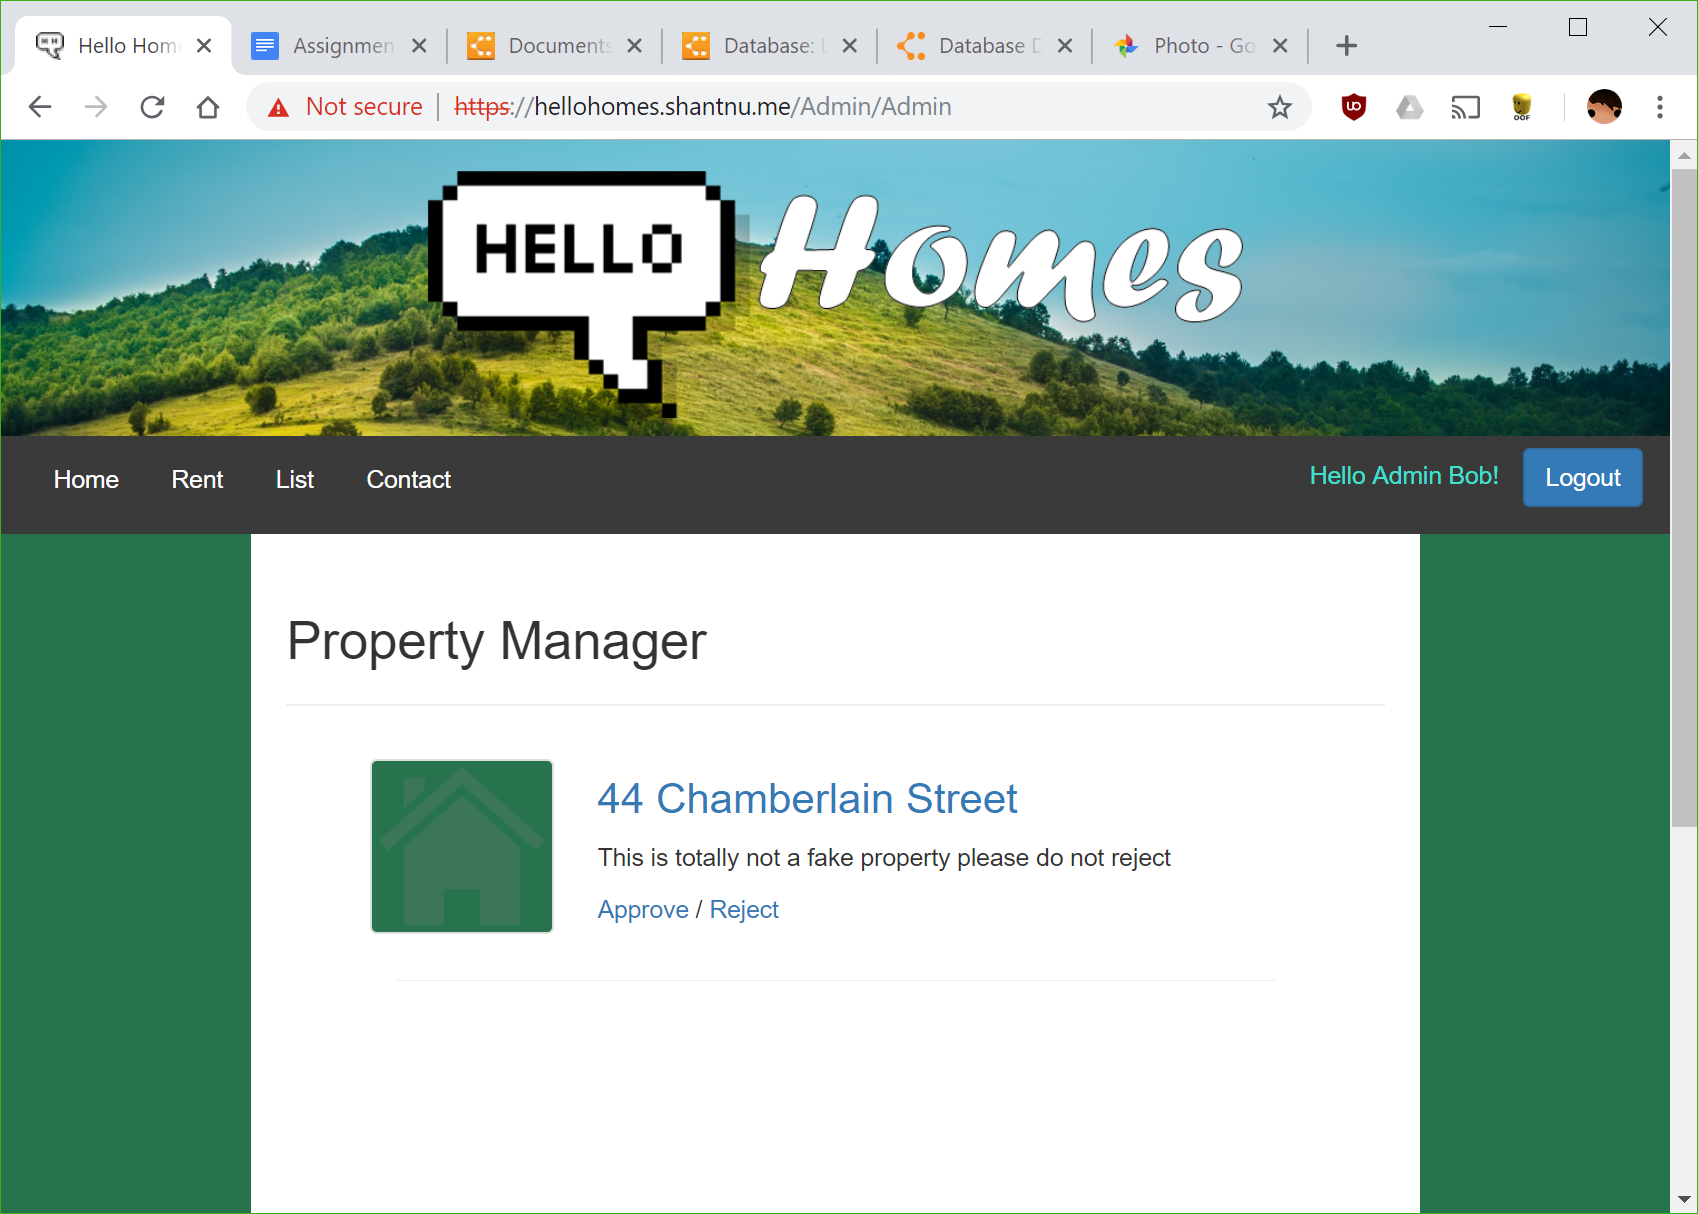
\includegraphics[width=0.7\textwidth]{figures/admin_page.png}
                \caption[Approve Property]{Admin viewing property listing for approval}
                \label{fig:admin_page}
            \end{figure}

            \begin{figure}[ht]
                \centering
                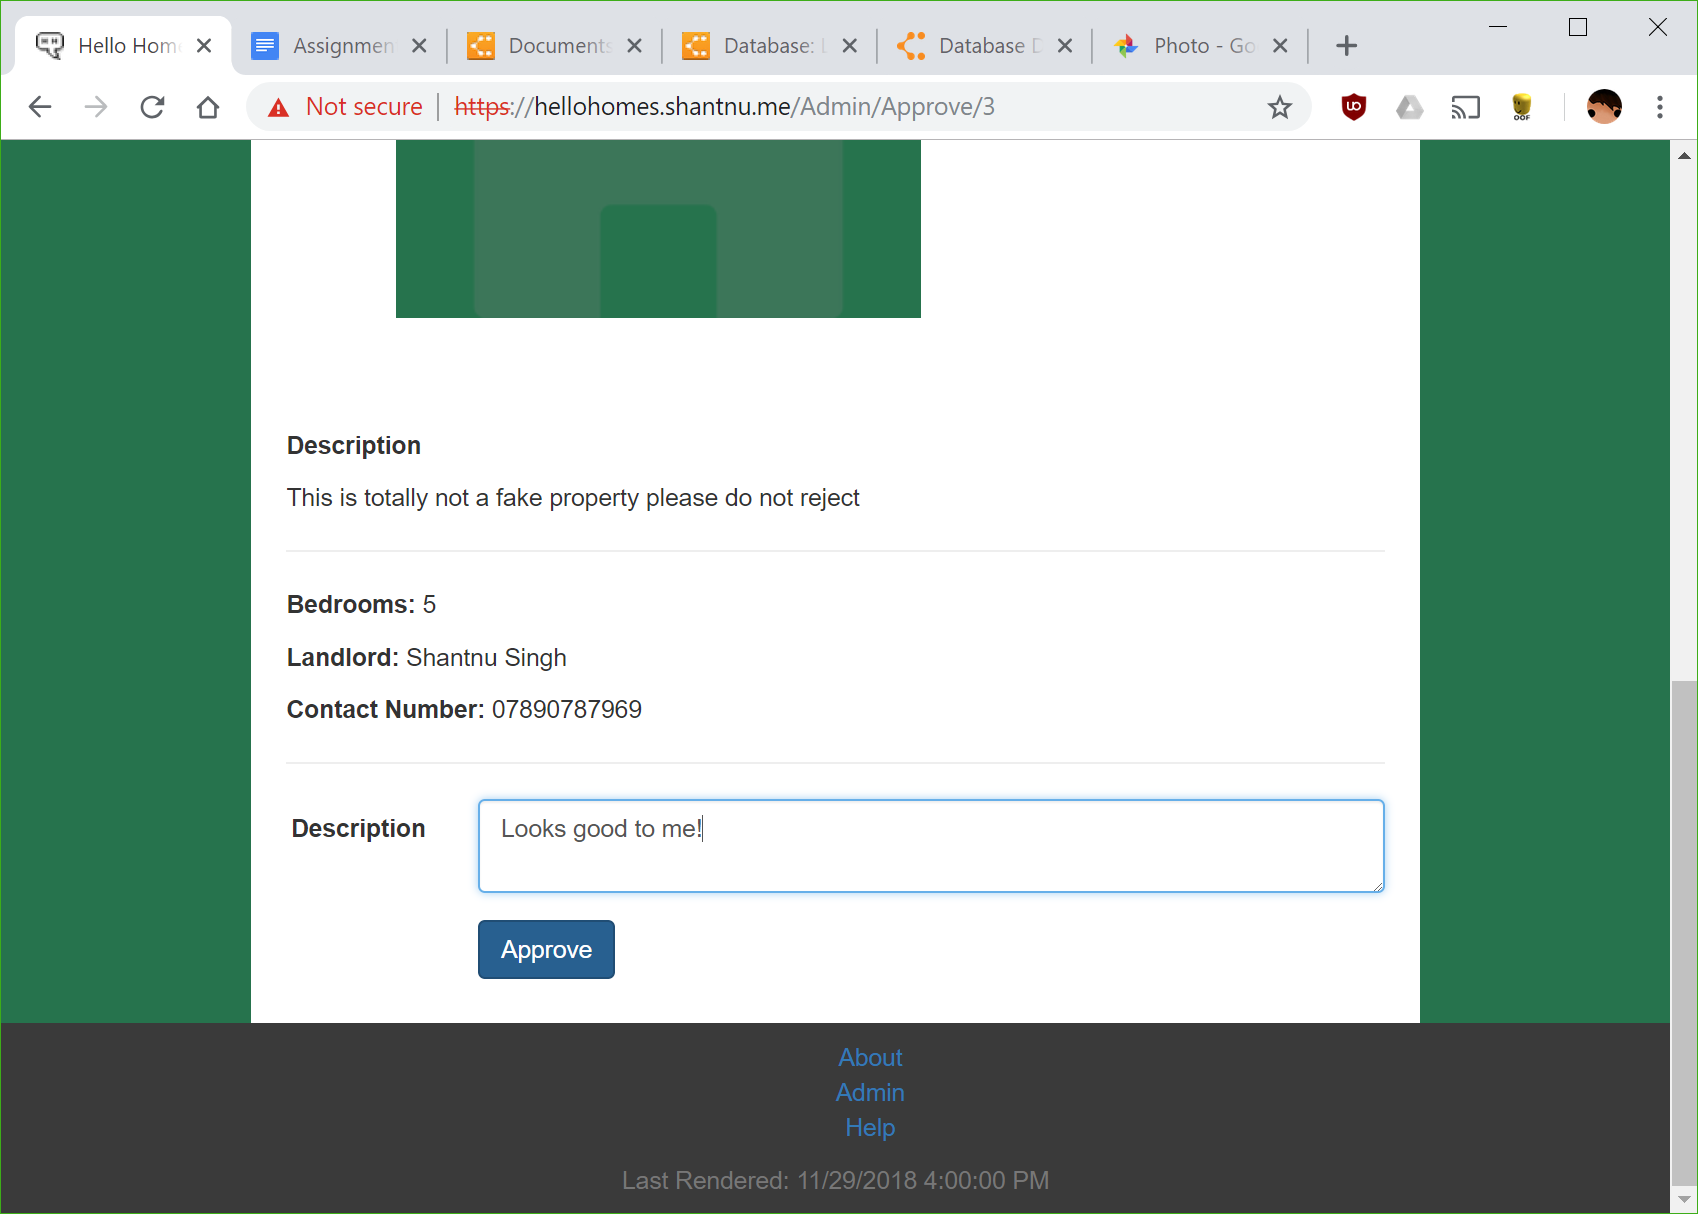
\includegraphics[width=0.7\textwidth]{figures/admin_approval.png}
                \caption[Comment on Property]{Admin approval or rejection comment}
                \label{fig:admin_approval}
            \end{figure}

        \par
            Only the landlord and admin have to be authenticated.
            This is done by adding authorisation to certain pages of the site, so that the user has to login before accessing them.
            There is provisioning for this in ASP.NET.
            When the user logs in, they are authenticated via details stored in the database and a cookie session is created.
            This cookie can be used to see which user is logged in throughout the session and to determine if they are allowed to view certain pages.

    \subsection{Additional Features}
        \par
            On top of the core functionality, we implemented some additional features to the site.
            These were done to demonstrate our understanding of Razor web development and to test its limitations.

        \par
            Firstly, we added the option to edit properties.
            If the user views a property they themself listed, the are shown a button on top of the page which allows them to edit the property.
            Doing this takes them to a page similar to the new property page, except the previous details are filled in.
            They can simply change any information and re-list the site.
            However, doing this means the approval status is reset.
            This was done to prevent a malicious landlord changing details after being approved, but to also allow them to act on the comments left by the admin.

        \par
            Since Razor pages allows \Csharp\space code to be run to pre-process a HTML page, we could use this to test some interesting features.
            On the homepage of the site, we display the “property of the day” and a “random property”.
            This is done by creating an array of all approved properties and choosing relevant ones for each section.
            For the property of the day, the result is based on the current day of the week and the number of approved properties, whereas the random property can be any approved property and changes upon refresh!

        \par
            We also experimented with routing and displaying data relevant to the user in the site.
            For example, clicking the user’s name on the navigation bar, next to the logout button, takes the user to their profile page where their details are visible.
            In the future, we could add the ability to edit profiles and maybe add a profile picture.

        \par
            A final example of additional features is embedding other services onto the website.
            On the contact page, we embedded a Google Maps applet which displays the location of the HelloHomes headquarters.
            Since HelloHomes is a fictional entity, we used the University’s address.

    \subsection{Security}
        \par
            Since we had done a number of cyber-security modules at the university, we thought it was important to consider the security aspects of the site.
            This also gave us the opportunity to evaluate the features provided by ASP.NET and Razor.

        \subsubsection{Password Hashing}
            \par
                Since the password had to be stored in an SQL database, we thought it was unwise to store them in plain text.
                This is especially important as, for example, Visual Studio has an option to view data stored in the database.
                Therefore, we implemented password hashing to the website.
                This is done by creating a SHA1 hash of the password before storing them to the database and then simply comparing the hash to a hashed version of the password entered by the user.
                The reason to use SHA1 was due to its superiority to MD5 and simplicity to some other algorithms.
                However, in the future we would like to implement PBKDF2 or bscript as they are the systems recommended in the field.

        \subsubsection{Secure File Upload}
            \par
                The only area of the site where the user could upload a file was when submitting an image along with the property.
                To combat this, we ensured the file input box only accepted image files with the MIME type for PNG or JPEG.
                This ensures that safe files are uploaded.
                To further improve this, the file size could be capped or the extension checked.

        \subsubsection{Built-in Security}
            \par
                There were a number of security features that were built into the libraries we used from ASP.NET.
                Firstly, since the user was authenticated via cookies, it was important that a malicious individual could not alter the value of the cookie to gain access to another user’s account.
                Fortunately, cookies are automatically hashed by ASP.NET’s authentication library and thus such an attack cannot be carried out.

            \par
                Secondly, Cross Site Request Forgery (CSRF) can be used to make malicious requests to the server from a user’s behalf.
                Razor pages come with built in verification to prevent this.

            \par
                Finally, when inputs are passed between the SQL database and the application, it is important to ensure they are sanitised to prevent SQL injection.
                Luckily, using the database context super-class when creating the database ensures this is done.
                This also protects the site against Cross-Site Scripting (XSS).


\section{Testing}

\section{Extensions}

\section{Critical Evaluation}

\begin{thebibliography}{1}
    \bibitem{cooper88}
        Cooper, R. and Kaplan, R.S., 1988. Measure costs right: make the right decisions. Harvard business review, 66(5), pp.96-103.
\end{thebibliography}

\end{document}
